\begin{frame}{WYSIWYG}

\begin{itemize}
\itemsep1pt\parskip0pt\parsep0pt
\item
  What You See Is What You Get

  \begin{itemize}
  \itemsep1pt\parskip0pt\parsep0pt
  \item
    Beispiele: Word/OpenOffice/Libreoffice
  \item
    Benutzer: Inhalt eingeben → Formatierung
  \item
    Programm: nach Umgebung → Layouting der Eingabe
  \item
    Prozess: nach und nach
  \end{itemize}
\item
  man legt fest, wie eine Überschrift \emph{aussieht}
\item
  man legt \emph{nicht} fest, was (strukturell!) eine Überschrift
  \emph{ist}
\item
  (aber: Formatvorlagen)
\end{itemize}

\end{frame}

\begin{frame}{WYSIWYM}

\begin{itemize}
\itemsep1pt\parskip0pt\parsep0pt
\item
  What You Get Is What You Mean
\item
  Auszeichnungssprachen: \emph{logische} Auszeichnung von
  \emph{Strukturen}
\item
  Beispiel: HTML

  \begin{itemize}
  \itemsep1pt\parskip0pt\parsep0pt
  \item
    Titel:
    \texttt{\textless{}title\textgreater{}Ich\ bin\ der\ Titel\textless{}/title\textgreater{}}
  \item
    kursiv:
    \texttt{\textless{}i\textgreater{}ich\ bin\ kursiv\textless{}/i\textgreater{}}
  \end{itemize}
\item
  Beispiel: \LaTeX
  \begin{itemize}
  \itemsep1pt\parskip0pt\parsep0pt
   \item 
    Titel:
    \texttt{\textbackslash{}title\{Ich\ bin\ auch\ ein\ Titel\}}
  \item
    kursiv:
    \texttt{\textbackslash{}textit\{und\ ich\ bin\ auch\ kursiv\}}
  \end{itemize}
\end{itemize}

\end{frame}

\begin{frame}{\LaTeX-Textsatz}

\begin{itemize}
\itemsep1pt\parskip0pt\parsep0pt
\item
  man legt fest, was vom Text z.B. eine Überschrift ist
\item
  man legt aber \emph{nicht} fest, wie eine Überschrift aussieht
\item
  Berufe: Typograph, Schriftsetzer, Designer
\item
  Vorgang: erst schreiben (Quelltext) und auszeichnen, dann layouten
  \emph{lassen}
\item
  \texttt{kompilieren}: Übersetzung vom Quelltext zum fertigen Dokument
\end{itemize}

\end{frame}

\begin{frame}{gefühlte Vorteile}

\begin{itemize}
\itemsep1pt\parskip0pt\parsep0pt
\item
  hochwertige Typographie (was bedeutet das??)
\item
  Dokumente sind leicht unterteilbar in einzelne Dateien
\item
  einfache Arbeit mit Referenzen und Zitierstilen
\item
  Sachen die in Word nicht funktioniert haben

  \begin{itemize}
  \itemsep1pt\parskip0pt\parsep0pt
  \item
    Bsp.: Pragmatikhandout: mehrfache Potenz. \LaTeX:
    \texttt{\textbackslash{}(\ a\^{}\{b\^{}\{c\^{}\{d\}\}\}\ \textbackslash{})}
  \end{itemize}
\item
  einfaches Aufschreiben von beliebig komplexen mathematischen Formeln
\item
  Text (besonders UTF-8) ist toll, weil universell und immer zugänglich
\end{itemize}

\end{frame}

\begin{frame}{Einarbeitungszeit}

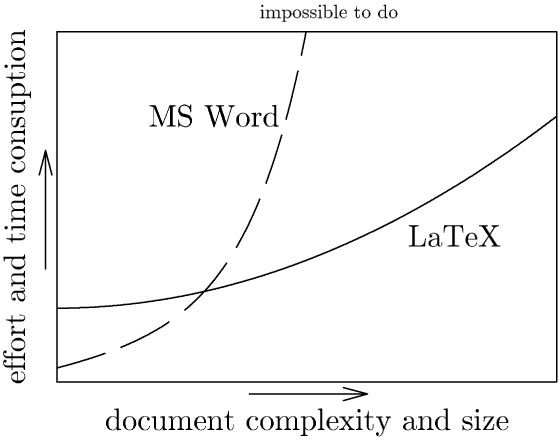
\includegraphics[width=\textwidth*0.8,height=\textheight*0.8,keepaspectratio]{../../img/miktex.png} Quelle:
\url{http://www.pinteric.com/miktex.html}

\end{frame}

\begin{frame}{Vorteile, die man später bemerkt}

\begin{itemize}
\itemsep1pt\parskip0pt\parsep0pt
\item
  Skalierbarkeit: „Bücher schreibt man in \LaTeX!``
\item
  kostenlos und bleibt es
\item
  Freiheit: keine Hersteller- bzw. Lizenzbindung (MS-Office-Preise,
  SPSS-Preise)
\item
  Akzeptanz \& Verbreitung

  \begin{itemize}
  \itemsep1pt\parskip0pt\parsep0pt
  \item
    kollaboratives Arbeiten ist leichter (jeder kann seinen Teil
    unabhängig einbinden)
  \item
    (Abschluss)arbeiten in der Mathematik, Naturwissenschaft und Technik
  \item
    Paper: \LaTeX-Templates von Journals
  \end{itemize}
\end{itemize}

\end{frame}

\begin{frame}{Nachteile}

\begin{itemize}
\itemsep1pt\parskip0pt\parsep0pt
\item
  schwieriger Einstieg
\item
  steilere Lernkurve
\item
  \ldots{} dafür gibt es dieses Seminar! Schildert mir Nachteile, die
  mir nicht einfallen)
\item
  Schriftarten (dafür gibt es aber \XeTeX \ und \LuaTeX \ usw.)
\end{itemize}

\end{frame}
